\section{Introduction}
Capturing individuals' responses, attitudes, and preferences effectively is the cornerstone of studying human subject studies, especially for the CSCW community. The effectiveness of eliciting these responses hinges upon the study protocol, survey mechanism, and design of the tool at hand~\cite{olsonWaysKnowingHCI2014, couperWebSurveyDesign2001, jackoHumancomputerInteractionHandbook2012}. While much research has explored the influence of the former two aspects, this research focuses on the design of a specific survey -- Quadratic Surveys. 

% TODO, for a cleaner thesis statement in the first par? mention challenges and interface here before diving deeper.

A~\textbf{Quadratic Survey} is a surveying tool that employs the quadratic mechanism. In this paper, we use the term~\textbf{Quadratic Mecahnism} to describe the mechanism where individuals express some intensity value bounded by a given budget using a quadratic formula.~\textbf{Quadratic Voting} (QV), also known as plural voting, is the most well-known application of this mechanism. Quadratic Voting allows participants to allocate a finite amount of credits across a list of options, voting multiple times to demonstrate their strength of approval, provided the quadratic cost remains within their given budget~\cite{lalley2018quadratic}. In this paper, we use the term~\textbf{Quadratic Survey} (QS) to focus on the surveys that use the quadratic mechanism to elicit individual preferences to gather public opinions. Recent work has demonstrated that QV can gauge public opinions~\cite{quarfoot2017quadratic} and can be transformed into surveys that outperform Likert scale surveys at eliciting individual preferences under resource-constrained scenarios~\cite{chengCanShowWhat2021}. 

The design of any response-capturing tool significantly influences individuals' abilities to express their attitudes. Political scientists have demonstrated that ballot designs alone can sway voter decisions~\cite{engstrom2020politics}, marketing and psychology researchers have examined how the presentation of questions influences responses~\cite{weijtersEffectRatingScale2010, kierujVariationsResponseStyle2010, toepoelSmileysStarsHearts2019}, and Human-Computer Interaction researchers have focused on evaluating and understanding web surveys and smart interfaces for surveys~\cite{farzandAestheticsEvaluatingResponse2024, xiaoTellMeYourself2020, pielotDidYouMisclick2024}. These studies highlight the importance of studying the interface and design for survey mechanisms.

Thus, the primary goal of this study is to present a novel interactive interface designed for quadratic surveys, which could presumably extend to other applications that utilize the quadratic mechanism. The Quadratic Mechanism is undeniably more complex than other voting and surveying mechanisms like the Likert scale survey~\cite{likertTechniqueMeasurementAttitudes1932}, where individuals select from a few responses, and Approval Voting~\cite{bramsApprovalVoting1978}, where participants mark as many options as they approve without constraints. Responding to a QS involves expressing numerical representations of a full set of constructed preferences. To mitigate such burden, the interface exploits human preference construction as Lichtenstein and Slovic~\cite{lichtensteinConstructionPreference2006} pointed out, when individuals do not have clear known preferences, they construct preferences in situ. This design involves scaffolding a two-step process involving an initial organization phase and a subsequent voting phase. \yhc{Yi-Hung: Exploits? Is it good or bad if human construct preferences in-situ when they do not have clear known preferences. What do you mean by exploitation here?}

Despite the advocacy of Quadratic Voting by Posner and Weyl~\cite{posner2018radical}, and its experimentation in various contexts such as the U.S. Colorado state government~\cite{ColoradoTriedNew}, the Democratic Caucus of the House of Representatives~\cite{QuadraticVotingColorado} in the U.S., government-sponsored hackathons~\cite{teamTaiwanDigitalMinister}, and the recent Gov4git~\cite{Gov4gitDecentralizedPlatform2023}, there is a notable gap that no peer-reviewed research has focused on the design perspective of such mechanisms. This increasing attention highlights the relevance and potential impact of QS. 

The importance of design in surveying tools, the growing usage of applications on the quadratic mechanism, and the lack of research on the design regarding quadratic mechanisms that one could apply, motivated our main research question: \textit{How can we design interactive interfaces to support participants in completing Quadratic Surveys?}

Quadratic Surveys and other quadratic mechanism powered applications allow individuals to allocate resources across multiple options, but the presence of many options can overwhelm participants, potentially compromising decision-making quality. Prior research in behavioral economics and marketing has pointed out the challenge of choice overload~\cite{iyengarWhenChoiceDemotivating2000} and overchoice~\cite{gourvilleOverchoiceAssortmentType2005}. It can be difficult for decision-makers to reduce the number of options present in a survey. At the same time, reducing cognitive load and making survey less challenging is critical if the survey designer ought to reduce survey response errors and provide `good enough' answers~\cite{lenznerCognitiveBurdenSurvey2010, blessAskingDifficultQuestions1992}. Effective design may mitigate these overload challenges, ensuring that the Quadratic Survey mechanism fulfills its potential to capture detailed and accurate preferences. Thus, more concretely, this study focused on answering the following three research questions:
\begin{itemize}
\item RQ1. How does the number of options on QS impact respondents' cognitive load?
\item RQ2a. How does the interactive interface involving grouping and direct manipulation interface influence QS respondents' cognitive load compared to text-based interface?
\item RQ2b. Across the two interfaces, what are the sources of cognitive load from?
\item RQ3. What are differences in QS respondents' behaviors when coping with long lists of options?
\end{itemize}

Before answering these research questions, we iteratively designed and built an interactive interface informed by prior literature in the questionnaire and survey response format. Then, we designed a two-by-two between-subject in-lab study where each group of participants experienced a QS with either a short or long list of options using a text-based or interactive-based interface. Participants' cognitive load was measured using NASA-TLX, a widely used assessment tool, followed by interviews. We recruited 41 participants from a Midwestern local community, asking participants their attitudes across a wide range of societal issues.

\paragraph{Contributions}
In this study, proposed an interactive interface for QS and highlighted the importance of using a two-step "organize then vote" interactive interface for QS surveys with long lists of options. While we were not able to show statistically significant differences in overall cognitive load (NASA-TLX scores) between text-based and interactive interfaces, qualitative interviews revealed a shift in cognitive load sources from operational causes in the text-based interface to strategic and higher-level causes in the interactive interface.  \yhc{might sound weak for the contributions when you presented the negative results first?} When there are more choices, the interactive interface allows for more frequent and incremental updates, supporting a more iterative and reflective decision-making process and indicating better engagement and understanding. This study also highlighted design recommendations for the use of QS and directions for the design of the quadratic mechanism. \yhc{Yi-Hung: Please ignore if it is a common sense in CSCW community. I am confused when I see these terms here. what do you mean by operational causes? and what do you mean by higher-level causes?}
% Highlight this is also the first work to investigate where people felt challenging when completing QS.

In the remainder of this paper, we focus on the related works in section~\ref{sec:relatedWorks}. Then, we detail the design decisions for the interactive QS interface, informed by the iterative design process and prior works, in section ~\ref{sec:interfaceDesign}. Experiment design follows in section~\ref{sec:experiment}. Study findings and discussion are presented in section~\ref{sec:result} and section~\ref{sec:discussion}.


% old tex lives here
% This challenge emphasizes the critical importance of designing and developing suitable interfaces for Quadratic Surveys to elicit truthful and in-depth preference information from respondents. Good design is essential; without it, the quality of collected data can suffer significantly. 
% These reasons strongly motivate  Addressing this question fills a important gap in the literature and enhances the practical utility of QS in capturing high-quality data across various applications.

% \begin{figure}[ht]
%     \centering
%     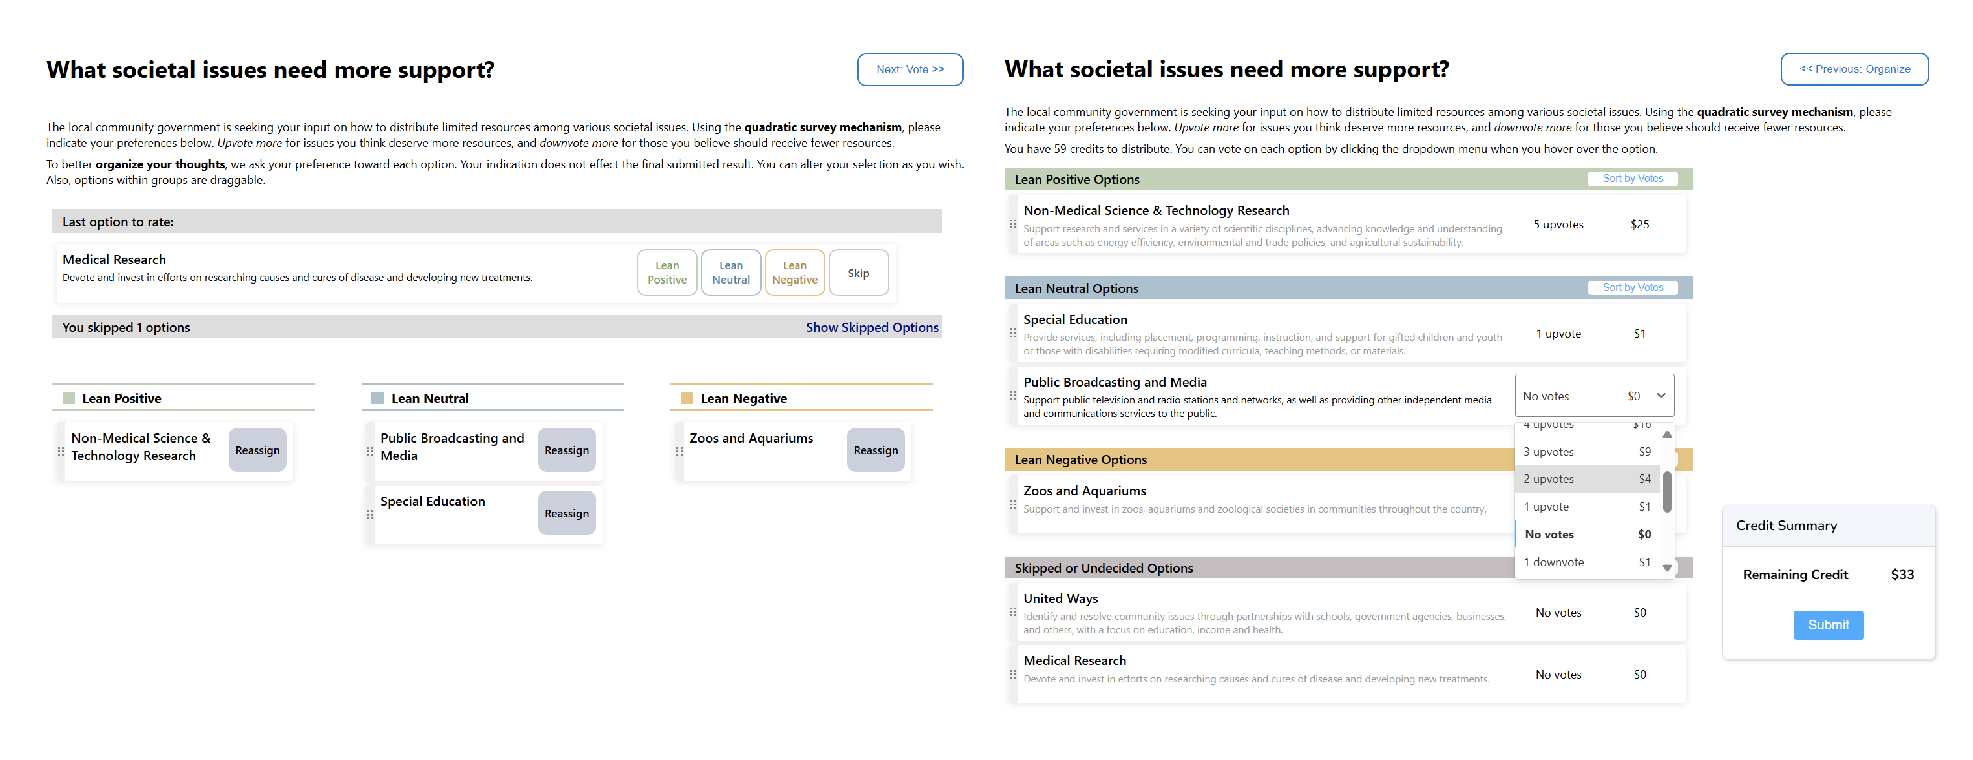
\includegraphics[width=\textwidth]{content/image/header.pdf}
%     \caption{We present an innovative interaction interface for Quadratic Survey}
%     \label{fig:header}
% \end{figure}
